\newpage
\def\thoigian{90}%--Thời gian
\de{Đề số 2}{Chương IV. Nguyên hàm - Tích phân}



\begin{center}
	\textbf{PHẦN 1 - CÂU TRẮC NGHIỆM BỐN PHƯƠNG ÁN}
\end{center}
\Opensolutionfile{ans}[ans/ans-TN-ONTAPCHUONG4-DE2]
%Câu 1- Nguyên hàm %[Dự án D - đợt 4 NH24-25- Hieu Hieu Minh Minh]
\begin{ex}%[2D4N1-1]%[Dự án D - đợt 4 NH24-25- Hieu Hieu Minh Minh]
	Hàm số $F(x)$ là một nguyên hàm của hàm số $f(x)$ trên khoảng $K$ nếu
	\choice
	{\True $F'(x)=f(x), \forall x \in K$}
	{$F'(x)=-f(x), \forall x \in K$}
	{$f'(x)=-F(x), \forall x \in K$}
	{$f'(x)=F(x), \forall x \in K$}
	\loigiai{Hàm số $F(x)$ là một nguyên hàm của hàm số $f(x)$ trên khoảng $K$ nếu $F'(x)=f(x)$, $\forall x \in K$.}
\end{ex}
%Câu 2 - Nguyên hàm
\begin{ex}%[2D4N1-4]%[Dự án D - đợt 4 NH24-25- Hieu Hieu Minh Minh]
	Gọi $F(x)$ là một nguyên hàm của hàm số $f(x)=\mathrm{e}^x$ thỏa mãn $F(0)=5$. Khẳng định nào sau đây là đúng?
	\choice
	{$F(x)=\mathrm{e}^x$}
	{\True $F(x)=\mathrm{e}^x+4$}
	{$F(x)=\mathrm{e}^x+5$}
	{$F(x)=\mathrm{e}^x-4$}
	\loigiai{Ta có
		\[\displaystyle \int \mathrm{e}^x\mathrm{d}x= \mathrm{e}^x+C.\]
		Vì $F(0)=5$ nên 
		\[F(0)=\mathrm{e}^0+C=5 \Leftrightarrow C=4.\]
		Vậy $F(x)=\mathrm{e}^x+4$.}
\end{ex}
%Câu 3 - Nguyên hàm
\begin{ex}%[2D4N1-4]%[Dự án D - đợt 4 NH24-25- Hieu Hieu Minh Minh]
	Họ nguyên hàm của hàm số $f(x)=7^x$ là
	\choice
	{$7^x+C$}
	{$7^x \ln 7+C$}
	{\True $\dfrac{7^x}{\ln 7}+C$}
	{$\dfrac{7^{x+1}}{x+1}+C$}
	\loigiai{
		Ta có $\displaystyle\int 7^x\mathrm{\,d}x=\dfrac{7^x}{\ln7}+C$.
	}
\end{ex}
%Câu 4 - Nguyên hàm
\begin{ex}%[2D4H1-1]%[Dự án D - đợt 4 NH24-25- Hieu Hieu Minh Minh]
	Hàm số $F(x)=x^2+\sin x$ là một nguyên hàm của hàm số
	\choice
	{$f(x)=2x-\cos x$}
	{$f(x)=\dfrac{1}{3} x^3-\cos x$}
	{$f(x)=\dfrac{1}{3} x^3+\cos x$}
	{\True $f(x)=2x+\cos x$}
	\loigiai{
		Ta có $f(x)=F'(x)=2x+\cos x$.
	}
\end{ex}

%Câu 5 - Tích phân
\begin{ex}%[2D4N2-1]%[Dự án D - đợt 4 NH24-25- Hieu Hieu Minh Minh]
	Cho hàm số $y=f\left( x \right)$ liên tục trên đoạn $\left[ a;b \right]$. Gọi $F\left( x \right)$ là một nguyên hàm của hàm số $f\left( x \right)$ trên đoạn $\left[ a;b \right]$. Khẳng định nào dưới đây là \textbf{sai}?
	\choice
	{$\displaystyle\int\limits_a^b{f\left( x \right)\mathrm{\,d}x}=F\left( b \right)-F\left( a \right)$}
	{\True $\displaystyle\int\limits_a^a{f\left( x \right)\mathrm{\,d}x}=1$}
	{$\displaystyle\int\limits_a^a{f\left( x \right)\mathrm{\,d}x}=0$}
	{$\displaystyle\int\limits_a^b{f\left( x \right)\mathrm{\,d}x}=-\displaystyle\int\limits_b^a{f\left( x \right)\mathrm{\,d}x}$}
	\loigiai{
		Ta có $\displaystyle\int\limits_a^a{f\left( x \right)\mathrm{\,d}x}=0$ nên $\displaystyle\int\limits_a^a{f\left( x \right)\mathrm{\,d}x}=1$ sai.
	}
\end{ex}

%Câu 6 - Tích phân
\begin{ex}%[2D4H2-1]%[Dự án D - đợt 4 NH24-25- Hieu Hieu Minh Minh]
	Cho hàm số $y=f(x)$ liên tục trên $\mathbb{R}$ thỏa mãn $\displaystyle\int\limits_0^6f(x) \mathrm{\,d}x=7$, $\displaystyle\int\limits_3^{10} f(x) \mathrm{\,d}x=8$, $\displaystyle\int\limits_3^6f(x) \mathrm{\,d}x=$ 9. Giá trị của $I=\displaystyle\int\limits_0^{10} f(x) \mathrm{\,d}x$ bằng
	\choice
	{$8$}
	{$5$}
	{\True $6$}
	{$7$}
	\loigiai{
		Ta có \allowdisplaybreaks
		\begin{eqnarray*}
			I&=&\displaystyle\int\limits_0^{10} f(x) \mathrm{\,d}x\\
			&=&\displaystyle\int\limits_0^3 f(x) \mathrm{\,d}x+\displaystyle\int\limits_3^{10} f(x) \mathrm{\,d}x\\
			&=&\left(\displaystyle\int\limits_0^6f(x) \mathrm{\,d}x-\displaystyle\int\limits_3^6f(x) \mathrm{\,d}x\right)+\displaystyle\int\limits_3^{10} f(x) \mathrm{\,d}x\\
			&=&(7-9)+8\\
			&=&6.
		\end{eqnarray*}
	}
\end{ex}
%Câu 7 - Tích phân
\begin{ex}%[2D4N2-1]%[Dự án D - đợt 4 NH24-25- Hieu Hieu Minh Minh]
	Cho hàm số $y=f(x)$ liên tục trên $\mathbb{R}$ và thỏa mãn $\displaystyle\int\limits_0^1f(x)\mathrm{\,d}x=-1$; $\displaystyle\int\limits_0^3f(x)\mathrm{\,d}x=5$. Giá trị của $\displaystyle\int\limits_1^3f(x)\mathrm{\,d}x$ bằng
	\choice
	{$4$}
	{$1$}
	{$5$}
	{\True $6$}
	\loigiai{
		Ta có $\displaystyle\int\limits_1^3f(x)\mathrm{\,d}x=\displaystyle\int\limits_0^3f(x)\mathrm{\,d}x-\displaystyle\int\limits_0^1f(x)\mathrm{\,d}x=5-(-1)=6$.
	}
\end{ex}
%Câu 8 - Tích phân
\begin{ex}%[2D4N2-1]%[Dự án D - đợt 4 NH24-25- Hieu Hieu Minh Minh]
	Cho hàm số $f(x)$ liên tục trên đoạn $[0; 3]$. Biết hàm số $F(x)$ là một nguyên hàm của hàm số $f(x)$ trên đoạn $[0; 3]$ và $F(0)=-1$, $F(3)=4$. Khi đó $\displaystyle\int\limits_0^3f(x)\mathrm{\,d}x$ bằng
	\choice
	{$3$}
	{$-4$}
	{$5$}
	{$-5$}
	\loigiai{
		Ta có $\displaystyle\int\limits_0^3f(x)\mathrm{\,d}x=F(3)-F(0)=4-(-1)=5$.
	}
\end{ex}

%Câu 9 - Ứng dụng hình học của tích phân 
\begin{ex}%[2D4N3-1]%[Dự án D - đợt 4 NH24-25- Hieu Hieu Minh Minh]
	Cho hàm số $y=f(x)$ liên tục trên $[1; 3]$. Diện tích hình phẳng giới hạn bởi đồ thị hàm số $y=f(x)$, trục hoành và các đường thẳng $x=1$, $x=3$ là
	\choice
	{\True $S=\displaystyle\int\limits_1^3|f(x)|\mathrm{\,d}x$}
	{$S=\displaystyle\int\limits_3^1|f(x)|\mathrm{\,d}x$}
	{$S=-\displaystyle\int\limits_1^3f(x)\mathrm{\,d}x$}
	{$S=\displaystyle\int\limits_1^3f(x)\mathrm{\,d}x$}
	\loigiai{
		Diện tích hình phẳng cần tính là $S=\displaystyle\int\limits_1^3|f(x)|\mathrm{\,d}x$.
	}
\end{ex}
%Câu 10 - Ứng dụng hình học của tích phân 
\begin{ex}%[2D4N3-3]%[Dự án D - đợt 4 NH24-25- Hieu Hieu Minh Minh]
	Thể tích của vật thể tròn xoay tạo thành khi quay hình phẳng giới hạn bởi các đường $y=x^2-2x$, $y=0$, $x=0$, $x=1$ quanh trục $Ox$ là
	\choice
	{$\dfrac{7\pi}{8}$}
	{$\dfrac{8\pi}{15}$}
	{$\dfrac{15\pi}{8}$}
	{$\dfrac{8\pi}{7}$}
	\loigiai{
		Ta có $V=\pi\displaystyle\int\limits_{0}^{1}\left(x^2-2x\right)^2\mathrm{\,d}x=\dfrac{8\pi}{15}$. 
	}
\end{ex}
%Câu 11 - Ứng dụng hình học của tích phân 
\begin{ex}%[2D4N3-3]%[Dự án D - đợt 4 NH24-25- Hieu Hieu Minh Minh]
	Cho hình phẳng $(H)$ giới hạn bởi đồ thị $y=2x-x^2$, trục hoành và hai đường thẳng $x=0$, $x=2$. Tính thể tích $V$ của khối tròn xoay sinh ra khi cho $(H)$ quay quanh trục $Ox$.
	\choice
	{$V=\pi \displaystyle\int\limits_0^2\left(2x-x^2\right)\mathrm{\,d}x$}
	{$V=\pi^2\displaystyle\int\limits_0^2\left(2x-x^2\right)^2d x$}
	{\True $V=\pi \displaystyle\int\limits_0^2\left(2x-x^2\right)^2\mathrm{\, d}x$}
	{$V=\displaystyle\int\limits_0^2\left(2x-x^2\right)^2 \mathrm{\, d} x$}
	\loigiai{Thể tích $V$ của khối tròn xoay sinh ra khi cho $(H)$ quay quanh trục $Ox$ là $V=\pi \displaystyle\int\limits_0^2\left(2x-x^2\right)^2 \mathrm{\, d} x$.}
\end{ex}
%Câu 12 - Ứng dụng hình học của tích phân 
\begin{ex}%[2D4N3-1]%[Dự án D - đợt 4 NH24-25- Hieu Hieu Minh Minh]
	Diện tích $S$ của hình phẳng giới hạn bởi đồ thị hàm số $y=x^2$, trục hoành $Ox$, các đường thẳng $x=1$, $x=2$ là
	\choice
	{$S=8$}
	{$S=\dfrac{8}{3}$}
	{$S=7$}
	{\True $S=\dfrac{7}{3}$}
	\loigiai{
		$S=\displaystyle\int\limits^2_1 x^2\mathrm{\,d}x=\dfrac{7}{3}$.
	}
\end{ex}
\Closesolutionfile{ans}
%\begin{center}
%	\textbf{ĐÁP ÁN}
%	\inputansbox{10}{ans/ans}	
%\end{center}

\begin{center}
	\textbf{PHẦN 2 - CÂU TRẮC NGHIỆM ĐÚNG SAI}
\end{center}
\setcounter{ex}{0}
\Opensolutionfile{ans}[ans/answer-DS-ONTAPCHUONG4-DE2]
%Câu 1%
\begin{ex}%[2D4H2-4]%[Dự án D - đợt 4 NH24-25- Hieu Hieu Minh Minh]
	Cho hàm số $f(x)$ và $g(x)$ liên tục trên $\mathbb{R}$ thỏa $\displaystyle\int\limits_{-3}^{0} f(x) \mathrm{\,d}x = -4$ và $\displaystyle\int\limits_{-3}^{0} g(x) \mathrm{\,d}x = -3$.
	\choiceTF
	{\True $\displaystyle\int\limits_{-3}^{0} [f(x)+g(x)] \mathrm{\,d}x = -7$} 
	{$\displaystyle\int\limits_{0}^{-3} f(x) \mathrm{\,d}x = -4$}
	{\True $\displaystyle\int\limits_{-3}^{0} -3f(x) \mathrm{\,d}x = 12$} 
	{Nếu $\displaystyle\int\limits_{-3}^{0} [mf(x)+ng(x)] \mathrm{\,d}x = -51$ và $\displaystyle\int\limits_{-3}^{0} [nf(x)+mg(x)] \mathrm{\,d}x = -19$ thì $m+n=-3$} 
	\loigiai{
		\begin{itemchoice}
			\itemch 
			$\displaystyle\int\limits_{-3}^{0} [f(x)+g(x)] \mathrm{\,d}x = \displaystyle\int\limits_{-3}^{0} f(x) \mathrm{\,d}x + \displaystyle\int\limits_{-3}^{0} g(x) \mathrm{\,d}x = (-4) + (-3) = -7$.	
			\itemch 
			Ta có $\displaystyle\int\limits_{0}^{-3} f(x) \mathrm{\,d}x = - \displaystyle\int\limits_{-3}^{0} f(x) \mathrm{\,d}x = -(-4) = 4$. 
			\itemch 
			$\displaystyle\int\limits_{-3}^{0} -3f(x) \mathrm{\,d}x = -3 \displaystyle\int\limits_{-3}^{0} f(x) \mathrm{\,d}x = -3 \cdot (-4) = 12$.
			\itemch 
			Ta có hệ phương trình
			\begin{eqnarray*}
				& & \heva{& m \displaystyle\int\limits_{-3}^{0} f(x)\mathrm{\,d}x + n \displaystyle\int\limits_{-3}^{0} g(x)\mathrm{\,d}x = -51 \\& n \displaystyle\int\limits_{-3}^{0} f(x)\mathrm{\,d}x + m\displaystyle\int\limits_{-3}^{0} g(x)\mathrm{\,d}x = -19}\\
				&\Leftrightarrow & \heva{& m(-4) + n(-3) = -51 \\& n(-4) + m(-3) = -19}\\
				&\Leftrightarrow & \heva{& 4m + 3n = 51 \\& 3m + 4n = 19}\\
				&\Rightarrow & 7m+7n=70\\
				&\Rightarrow & m+n=10.
			\end{eqnarray*}	
		\end{itemchoice}			
	}
\end{ex}
%Câu 2%
\begin{ex}%[2D4V3-1]%[Dự án D - đợt 4 NH24-25- Hieu Hieu Minh Minh]
	Cho hàm số $y=f(x)=\sqrt{x}$ có đồ thị $(C)$. Gọi $D$ là hình phẳng giới hạn bởi đồ thị $(C)$, trục hoành và đường thẳng $x=4$.
	\choiceTF
	{\True Diện tích hình phẳng $D$ là $S=\displaystyle\int\limits_{0}^4\sqrt{x}\mathrm{\,d}x$}
	{Thể tích khối tròn xoay khi quay hình phẳng $D$ quanh trục $Ox$ là $V=\displaystyle\int\limits_{0}^4 x \mathrm{\,d}x$}
	{Gọi $S_1$ là diện tích hình phẳng giới hạn bởi đồ thị $(C)$, đường thẳng $d\colon y=-x+2$. Khi đó $S_1=\dfrac{4}{3}\sqrt{2}-2$}
	{Đường thẳng $x=a$, ($0 < a < 4$) chia hình phẳng $D$ thành hai phần có diện tích bằng nhau. Khi đó $a=\sqrt[3]{2}$}
	\loigiai{
		\begin{itemchoice}
			\itemch 
			Diện tích hình phẳng $D$ là $S=\displaystyle\int\limits_{0}^4 \sqrt{x} \mathrm{\,d}x$.
			\itemch
			Thể tích khối tròn xoay khi quay hình phẳng $D$ quanh trục $Ox$ là $V=\pi\displaystyle\int\limits_{0}^4 x \mathrm{\,d}x$.
			\itemch 
			Diện tích hình phẳng giới hạn bởi đồ thị $(C)$, đường thẳng $d\colon y=-x+2$ và trục hoành là
			\[S=\displaystyle\int\limits_{0}^1 \sqrt{x} \mathrm{\,d}x + \displaystyle\int\limits_{1}^2 \left(-x+2\right) \mathrm{\,d}x =\dfrac{2}{3} \sqrt{x^3} \biggl|_{0}^{1}  + \left(-\dfrac{x^2}{2}+2x\right) \biggl|_{1}^{2}=\dfrac{7}{6}.\]
			\itemch 
			Ta có \\
			$S = \displaystyle\int\limits_{0}^{4} \sqrt{x} \mathrm{\,d}x = \displaystyle\int\limits_{0}^{4} x^{\frac{1}{2}} \mathrm{\,d}x = \dfrac{2}{3} \sqrt{x^3} \biggl|_{0}^{4} = \dfrac{16}{3}$.\\
			$S_2 = \displaystyle\int\limits_{0}^{a} \sqrt{x} \mathrm{\,d}x =  \dfrac{2}{3} \sqrt{x^3} \biggl|_{0}^{a} = \dfrac{2}{3}\sqrt{a^3}$.\\
			Đường thẳng $x=a$ ($0 < a < 4$) chia $D$ thành hai phần có diện tích bằng nhau nên 
			\begin{eqnarray*}
				S_2 = \dfrac{S}{2} &\Leftrightarrow& \dfrac{2}{3} \sqrt{a^3} = \dfrac{8}{3} \\
				&\Leftrightarrow& \sqrt{a^3} = 4 \\
				&\Leftrightarrow& a^3 = 16 \Leftrightarrow a = 2\sqrt[3]{2}.
			\end{eqnarray*}
			
			
		\end{itemchoice}
	}
\end{ex}
\Closesolutionfile{ans}
%\inputansbox[2]{2}{ans/answer.tex}

\begin{center}
\textbf{PHẦN 3 - CÂU TRẮC NGHIỆM TRẢ LỜI NGẮN}
\end{center}
\setcounter{ex}{0}
\Opensolutionfile{ans}[ans/ans-KQ-ONTAPCHUONG4-DE2]
%Câu 1%
\begin{ex}%[2D4H2-3]%[Dự án D - đợt 4 NH24-25- Hieu Hieu Minh Minh]
	Kết quả của tích phân $\displaystyle\int\limits_0^{\tfrac{\pi}{4}} \sin x\mathrm{\,d}x = \dfrac{a-\sqrt{b}}{2}$. Tính $a+b$.
	\shortans{4}
	\loigiai{
		Ta có $\displaystyle\int\limits_0^{\tfrac{\pi}{4}} \sin x\mathrm{\,d}x = -\cos x\Bigg|_0^{\tfrac{\pi}{4}} = \left(-\cos\dfrac{\pi}{4}\right)-(-\cos 0)=-\dfrac{\sqrt{2}}{2}-(-1)=\dfrac{2-\sqrt{2}}{2}$.\\
		Vậy $a+b=2+2=4$.
	}
\end{ex}
%Câu 2%
\begin{ex}%[2D4V2-6]%[Dự án D - đợt 4 NH24-25- Hieu Hieu Minh Minh]
	\immini[thm]{Một vật chuyển động trong $7$ giờ với vận tốc $v$ (km/h) phụ thuộc vào thời gian $t$ (h) có đồ thị là một phần của đường parabol có đỉnh $I(3;9)$ và trục đối xứng song song với trục tung như hình bên phải. Tính quãng đường mà vật di chuyển được trong $7$ giờ (làm tròn kết quả đến phần mười).}{
		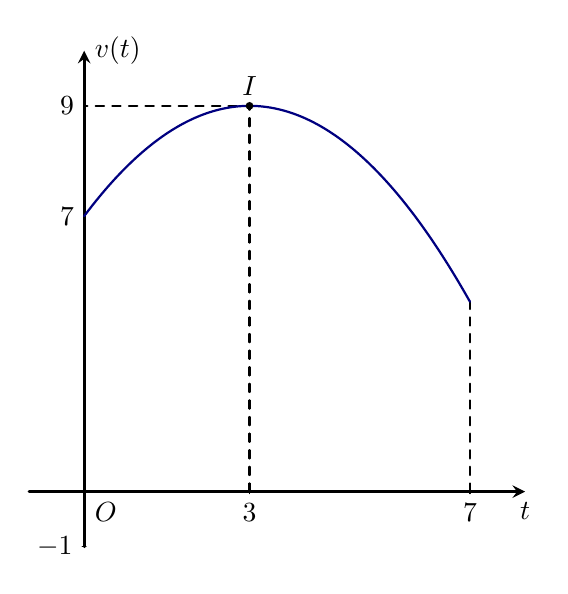
\begin{tikzpicture}[scale = 0.7,line join = round, line cap = round,>=stealth,thick,x = 1cm,y = 1cm] 
			%Vẽ hệ trục Oxy 
			\draw[->,line width = 1pt] (-1,0)--(0,0) node[below right]{$O$}--(8,0) node[below]{$t$}; 
			\draw[->,line width = 1pt] (0,-1)--(0,8) node[right]{$v(t)$}; 
			%Vẽ các điểm trên hệ trục 
			\foreach \x in {3,7} \draw[thin] (\x,1pt)--(\x,-1pt) node [below] {$\x$}; 
			\node[left] at (0,5) {$7$};
			\draw [dashed] (3,0)--(3,7) node[above]{$I$}--(0,7) node[left]{$9$};
			\draw [dashed] (7,0)--(7,3.45);
			\foreach \y in {-1} \draw[thin] (1pt,\y)--(-1pt,\y) node [left] {$\y$}; 
			%Vẽ đồ thị hàm số 
			\draw[samples=200,domain=0:7,smooth,blue!50!black] plot (\x, {-2/9*(\x-3)^2+7}); 
			\fill[black] (3,7) circle (2pt);
	\end{tikzpicture}}
	\shortans{56{,}3}
	\loigiai{
		Giả sử phương trình đường parabol $(P)$ là $v = at^2 + bt + c, (a \neq 0)$.\\
		Parabol $(P)$ có đỉnh là $I(3;9)$, đồng thời đi qua điểm \( (0;7) \) nên ta có hệ phương trình\\
		\[\heva{&9a+3b+c=9\\&c=7\\&-\dfrac{b}{2a}=3}\Leftrightarrow \heva{&a=-\dfrac{2}{9}\\&b=\dfrac{4}{7}\\&c=7}\Rightarrow (P)\colon v=-\dfrac{2}{9}t^2+\dfrac{4}{7}t+7.\]
		Vậy quãng đường vật di chuyển trong thời gian $7$ giờ là\\
		\[S = \displaystyle\int\limits_{0}^{7} \left(-\dfrac{2}{9}t^2+\dfrac{4}{7}t+7\right) \mathrm{\,d}t=\dfrac{1519}{27}\approx 56{,}3 \text{ (km)}.\]
	}
\end{ex}
%Câu 3%
\begin{ex}%[2D4H3-1]%[Dự án D - đợt 4 NH24-25- Hieu Hieu Minh Minh]
	Gọi $(H)$ là hình phẳng giới hạn bởi đồ thị $y=x^2$, trục hoành và hai đường thẳng $x=1$, $x=2$. Biết diện tích $S$ của hình phẳng $(H)$ là $S=\dfrac{a}{b}$ (với $a$, $b\in \Bbb{N}$ và $\dfrac{a}{b}$ tối giản). Tính $a+b$.
	\shortans{$10$}
	\loigiai{
		Diện tích $S$ của hình phẳng $(H)$ là $S=\displaystyle\int\limits_1^2|x^2|\mathrm{\,d}x=\displaystyle\int\limits_1^2 x^2\mathrm{\,d}x=\dfrac{x^3}{3}\Bigg|_1^2=\dfrac{7}{3}$.\\
		Suy ra $a=7$, $b=3$.\\
		Vậy $a+b=7+3=10$.
	}
\end{ex}
%Câu 4%
\begin{ex}%[2D4V3-3]%[Dự án D - đợt 4 NH24-25- Hieu Hieu Minh Minh]
	\immini[thm]{
		Một chậu cây có chiều cao là $30$ cm và đường kính miệng chậu là $30$ cm. Mặt cắt ngang của chậu cây là một đường parabol (tham khảo hình vẽ). Tính thể tích của chậu cây đó (đơn vị: $\mathrm{dm}^3$, kết quả làm tròn đến hàng phần chục).
		\shortans[]{$10{,}6$}
	}{
		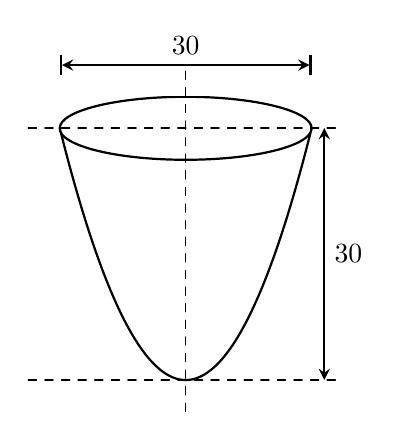
\begin{tikzpicture}[line join=round, line cap=round,>=stealth,thick,scale=0.8]
			\tikzset{label style/.style={font=\footnotesize}}
			\draw[dashed,thin](-2.5,0)--(2.5,0);
			\draw[dashed,thin](-2.5,4)--(2.5,4);
			\draw[dashed,thin](0,-0.5)--(0,5);
			\draw[<->](2.2,0)--(2.2,4)node[midway,right]{$30$};
			\draw[|<->|](-2,5)--(2,5)node[midway,sloped,above]{$30$};
			\begin{scope}
				\clip (-2.5,-0.5) rectangle (2.5,4.5);
				\draw (-2,4) plot[samples=200,domain=-2:2,smooth,variable=\x] (\x,{1*(\x)^2+0*(\x)+0}) arc(0:360:2 cm and 0.5 cm);
			\end{scope}
		\end{tikzpicture}
	}
	\loigiai{
		\immini{
		Gắn hệ trục tọa độ như hình.\\
		Vì parabol đi qua gốc tộ độ $O$ nên $(P):y=ax^2$.\\
		Vì parabol đi qua điểm $(15;30)$ nên $a=\dfrac{y}{x^2}=\dfrac{30}{15^2}=\dfrac{2}{15}$.\\
		Suy ra parabol $(P):y=\dfrac{2}{15}x^2\Rightarrow x^2=\dfrac{15}{2}y$.\\
		Chậu cây được tạo ra khi quay parabol xung quanh trục $Oy$, giới hạn bởi các đường thẳng $y = 0$, $y = 30$.\\
		Thể tích chậu cây là
		\[V=\pi \displaystyle\int\limits_0^{30}\left(\dfrac{15}{2} y\right) \mathrm{\,d}y=3375\pi\ \left(\mathrm{cm}^3\right)\approx 10{,}6\ \left(\mathrm{dm}^3\right). \]}{
		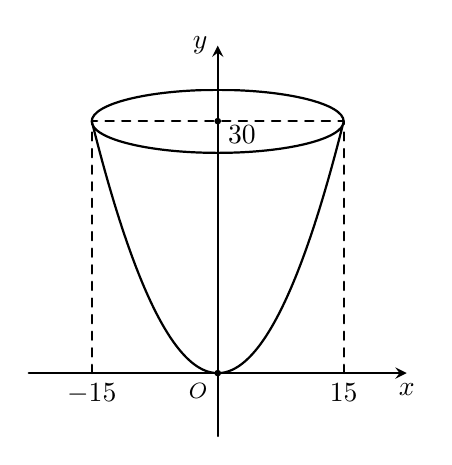
\begin{tikzpicture}[line join=round, line cap=round,>=stealth,thick,scale=0.8]
			\tikzset{label style/.style={font=\footnotesize}}
			\draw[->] (0,-1)--(0,5.2)node[left]{$y$};
			\draw[->] (-3,0)--(3,0)node[below]{$x$};
			\fill (0,0) node[below left]{\footnotesize $O$} circle(1.5pt);
			\draw[dashed,thin](-2.5,0)--(2.5,0);
			\draw[dashed,thin](0,-0.5)--(0,5);
			\draw[dashed](2,0)node[below]{$15$}--(2,4)--(0,4);
			\draw[dashed](-2,0)node[below]{$-15$}--(-2,4)--(0,4);
			\node[below right] at (0,4.1){$30$};
			\fill (0,4) circle(1.5pt);
			\begin{scope}
				\clip (-2.5,-0.5) rectangle (2.5,4.5);
				\draw (-2,4) plot[samples=200,domain=-2:2,smooth,variable=\x] (\x,{1*(\x)^2+0*(\x)+0}) arc(0:360:2 cm and 0.5 cm);
			\end{scope}
		\end{tikzpicture}
		}
	}
\end{ex}

\Closesolutionfile{ans}


\begin{center}
	\textbf{PHẦN 4 - TỰ LUẬN}
\end{center}
%Câu 1%
\begin{bt}%[2D4H2-1]%[Dự án D - đợt 4 NH24-25- Hieu Hieu Minh Minh]
	Biết $F(x)$ là một nguyên hàm của hàm số $f(x)=\sin x$ và $F(0)=1$. Tính $F \left(\dfrac{\pi}{2}\right)$.
	\loigiai{Vì $F(x)$ là một nguyên hàm của hàm số $f(x)=\sin x$ nên
		$$F\left(\dfrac{\pi}{2}\right)-F(0)=\displaystyle \int \limits_{0}^{\frac{\pi}{2}} f(x) \mathrm{\,d}x.$$
		Do đó $F\left(\dfrac{\pi}{2}\right)=F(0)+ \displaystyle \int \limits_{0}^{\frac{\pi}{2}} f(x) \mathrm{\,d}x=1+\displaystyle \int \limits_{0}^{\frac{\pi}{2}} \sin x \mathrm{\,d}x=1+1=2$.
	}
\end{bt} 
%Câu 2%
\begin{ex}%[2D4V2-3]%[Dự án D - đợt 4 NH24-25- Hieu Hieu Minh Minh]
	Cho $\displaystyle\int\limits_0^{\tfrac{\pi}{4}} \left(\tan^2x+\sin^2\dfrac{x}{2}\right)\mathrm{\,d}x=a+\dfrac{\pi}{b}-\dfrac{\sqrt{c}}{4}$ (với $a$, $b$, $c\in \Bbb{Z}$). Tính giá trị của biểu thức $S=a+b-3c$.
	\shortans{$-13$}
	\loigiai{
		Ta có 
		\begin{eqnarray*}
			\displaystyle\int\limits_0^{\tfrac{\pi}{4}} \left(\tan^2x+\sin^2\dfrac{x}{2}\right)\mathrm{\,d}x&=&\displaystyle\int\limits_0^{\tfrac{\pi}{4}} \left(\dfrac{1}{\cos^2x}-1+\dfrac{1-\cos x}{2}\right)\mathrm{\,d}x\\
			&=&\displaystyle\int\limits_0^{\tfrac{\pi}{4}} \left(\dfrac{1}{\cos^2x}-\dfrac{1}{2}\cos x-\dfrac{1}{2}\right)\mathrm{\,d}x\\
			&=&\left(\tan x-\dfrac{1}{2}\sin x-\dfrac{1}{2}x\right)\Bigg|_0^{\tfrac{\pi}{4}}\\
			&=&1-\dfrac{\sqrt{2}}{4}-\dfrac{\pi}{8}\\
			&=&1+\dfrac{\pi}{-8}-\dfrac{\sqrt{2}}{4}.
		\end{eqnarray*}
		Suy ra $a=1$, $b=-8$, $c=2$.\\
		Vậy $a+b-3c=1-8-3\cdot 2=-13$.
	}
\end{ex}
%Câu 3%
\begin{ex}%[2D4V3-5]%[Dự án D - đợt 4 NH24-25- Hieu Hieu Minh Minh]
	\immini{Một gia đình muốn làm cái cổng như hình bên. Phần phía trên cổng có hình dạng là một parabol với $IH = 2,5\,\text{m}$, phần phía dưới là một hình chữ nhật có kích thước $AD = 4\,\text{m}$, $AB = 6\,\text{m}$. Giả sử giá để làm phần cổng được tô màu (phần hình chữ nhật $ABCD$) là $900\,000\,\text{đ/m}^2$ và giá để làm phần cổng phía trên là $1\,300\,000\,\text{đ/m}^2$. Tính số tiền gia đình đó phải trả là bao nhiêu triệu đồng?}{
		\begin{tikzpicture}[scale=0.6] 
			\coordinate (D) at (0, 0);
			\coordinate (C) at (6, 0);
			\coordinate (A) at (0, 4);
			\coordinate (B) at (6, 4);
			\coordinate (H) at (3, 4); % Trung điểm AB
			\coordinate (I) at (3, 4 + 2.5); % Đỉnh parabol
			\draw[step=1, gray!50, very thin] (-0.5, -0.5) grid (6+0.5, 4+2.5+0.5);
			\draw[blue, thick, fill=green!40] (D) -- (A) -- (B) -- (C) -- cycle;
			\draw[blue, thick] (A) parabola bend (I) (B);
			\draw[blue, thick] (I) -- (H);
			\node[left=2pt] at (0, 4/2) {\(4m\)}; % Giữa AD
			\node[below=2pt] at (6/2, 0) {\(6m\)}; % Giữa DC
			\node[right=2pt] at (6/2, 4 + 2.5/2) {\(2{,}5m\)}; % Giữa IH (dùng dấu phẩy)
			\foreach \i/\g in {A/135,B/45,C/45,D/135,I/90,H/-90}{\draw[fill=black](\i) circle (1.5pt) ($(\i)+(\g:5mm)$) node[scale=1]{$\i$};}
		\end{tikzpicture}
	}
	
	\shortans{$34{,}6$}
	\loigiai{
		\begin{center}
			
			\begin{tikzpicture}[scale=0.6] 
				\coordinate (D) at (0, 0);
				\coordinate (C) at (6, 0);
				\coordinate (A) at (0, 4);
				\coordinate (B) at (6, 4);
				\coordinate (H) at (3, 4); % Trung điểm AB
				\coordinate (I) at (3, 4 + 2.5); % Đỉnh parabol
				\draw[step=1, gray!50, very thin] (-0.5, -0.5) grid (6+0.5, 4+2.5+0.5);
				\draw[blue, thick, fill=green!40] (D) -- (A) -- (B) -- (C) -- cycle;
				\draw[blue, thick] (A) parabola bend (I) (B);
				\draw[blue, thick] (I) -- (H);
				\node[left=2pt] at (0, 4/2) {\(4m\)}; % Giữa AD
				\node[below=2pt] at (2, 0) {\(6m\)}; % Giữa DC
				\node[right=2pt] at (6/2, 4 + 2.5/2) {\(2{,}5m\)}; % Giữa IH (dùng dấu phẩy)
				
				\coordinate (A1) at (-1.5, 4);
				\coordinate (B1) at (7.5, 4);
				
				\draw[->, thick] (A1) -- (B1) node[anchor=north east]{$x$};
				\coordinate (K) at (3, -1);
				\coordinate (T) at (3, 8);
				\draw[->, thick] (K) -- (T) node[anchor=north east]{$y$};
				\foreach \i/\g in {A/135,B/45,C/45,D/135,I/60,H/-45}{\draw[fill=black](\i) circle (1.5pt) ($(\i)+(\g:6mm)$) node[scale=1]{$\i$};}
			\end{tikzpicture}
		\end{center}
		Phần phía trên cổng $(P)$ có dạng $ y = ax^2 + bx + c $ ($a \neq 0$).\\
		Vì $(P)$ đi qua điểm $ I(0; 2,5) $, $ A(-3; 0) $, $ B(3; 0) $ nên ta có hệ 
		$\heva{&9a + 3b + c = 0 \\ &9a - 3b + c = 0 \\ &c = 2{,}5} \Leftrightarrow \heva{& a = -\dfrac{5}{18} \\ &b = 0 \\ &c = 2{,}5.}$\\
		Do vậy $(P)\colon y = -\dfrac{5}{18}x^2 + 2{,}5$. \\
		Diện tích phần phía trên cổng là $ S_1 = \displaystyle\int_{-3}^{3} \left| -\dfrac{5}{18}x^2 + 2{,}5 \right| \mathrm{d}x = 10$ (m$^2$). \\
		Diện tích phần phía dưới là $ S_2 = 4 \cdot 6 = 24$ (m$^2$). \\
		Số tiền phải trả là $ 10 \cdot 1\,300\,000 + 24 \cdot 900\,000 = 13\,000\,000 + 21\,600\,000 = 34\,600\,000 $ đồng hay số tiền phải trả là $34{,}6$ triệu đồng. 		
	}
\end{ex}
